\chapter{Fundamentação Teórica}
\label{chap:fundteor}

\section{Inteligência artificial e algoritmos de busca}
\label{ia_algoritmos_de_busca}
Na medida em que o mundo se torna mais complexo, novas técnicas de resolução de problemas são necessárias. Nesse sentido, a \gls*{ia} vem sendo de grande ajuda: atividades que duram dias para um ser humano comum realizar podem ser finalizadas em apenas alguns segundos por um computador. Desde diagnósticos de doenças raras à concepção do carro autônomo, a IA está se tornando cada vez mais uma realidade.

O objetivo principal das técnicas de inteligência artificial é construir agentes inteligentes que agem de forma racional. Segundo \citeonline[p.~5]{Winston92}, “Inteligência artificial é o estudo de computações que permitem perceber, raciocinar e agir”. Sobre essa ótica, as máquinas devem ser capazes de tomar diferentes decisões, com base em suas próprias experiências.

Boa parte dos problemas que podem ser resolvidos com IA podem ser caracterizados como um “problema de busca”. Planejamento de rotas, ordenação, navegação de robôs e resolução de quebra-cabeças são alguns dos vários exemplos que podem ser citados. Todos esses problemas possuem a mesma estrutura e consistem de: um espaço de estados, um estado inicial e um objetivo final. O espaço de estados é o conjunto de todos os estados em que se pode estar. O estado inicial é onde a busca se inicia. E, por fim, o objetivo final é onde se quer chegar \cite{Akhtar2019}.

Durante a realização de uma busca, diversas possibilidades de ações a serem tomadas podem estar disponíveis ao mesmo tempo (virar à esquerda, direita, ou seguir em frente, por exemplo). O papel do algoritmo é analisar todas as possibilidades para conseguir definir a sequência de ações que fará o agente sair do estado inicial até o objetivo final. Em determinadas situações, cada ação pode estar associada também à um custo. Dessa forma, a maior parte dos agentes inteligentes irá procurar não só o objetivo final, mas também a melhor forma de se chegar até ele \cite{Endriss2015}.

Usualmente, o espaço de estados pode ser representado por nós, onde cada nó é um estado. A representação dos nós varia a depender do problema. No contexto de planejamento de rotas, os nós são as posições no mapa, por exemplo. Para a resolução de um labirinto, o espaço de estados pode ser representado por uma matriz, onde cada célula da matriz é uma posição do labirinto em que o agente pode estar.

Grande parte dos algoritmos de busca podem ser adaptados para a resolução de um labirinto. Porém, conforme demonstrado por \citeonline{Tjiharjadi2017}, destacam-se: Flood Fill e A*. O A*, por sua vez, pode ser considerado uma derivação do algoritmo de Dijkstra.

\subsection{Algoritmo de Dijkstra}
\label{ssec:algoritmo_dijkstra}
O método de Dijkstra foi concebido em 1956 por Edsger W. Dijkstra. Foi um dos primeiros a serem publicados. Nele, inicialmente, considera-se todos os nós como não visitados. Atribui-se valor zero para a estimativa de custo do nó inicial e infinito para todos os outros nós. Em seguida, é calculada a estimativa de custo de deslocamento para todos os nós vizinhos, passando pelo nó atual. O nó atual é marcado como “visitado” e o mesmo processo é repetido para o próximo nó vizinho, que possui o menor custo. O próximo nó terá a sua estimativa de custo somada com a do nó anterior (caso a soma seja menor do que a estimativa de custo já associada a ele), uma vez que para chegar até ele houve um custo associado. Nós que já foram visitados nunca serão checados novamente. O processo é repetido até que o nó final seja alcançado.

\subsection{Algoritmo A*}
\label{ssec:aestrela}
A* (pronunciado A-estrela) foi publicado inicialmente por Peter Hart, Nils Nilsson e Bertram Raphael em 1968. Seus criadores provaram que tal método garante que um caminho será encontrado, se o mesmo existir \cite{Hart1968}. Pode ser considerado como uma extensão do algoritmo de Dijkstra, utilizando heurística para melhorar sua performance.

Nele, são utilizadas duas listas: aberta e fechada. A lista aberta é composta pelos nós que foram visitados, mas não expandidos. Ou seja: os vizinhos ainda não foram explorados. Pode ser considerada como uma lista de pendências. A lista fechada consiste nos nós que que foram visitados e já expandidos.

O algoritmo procura minimizar $f(n) = g(n) + h(n)$, onde $g(n)$ é o custo do inicio do caminho até o nó atual e h(n) é a função heurística que estima o menor custo do nó atual até o objetivo. 
Inicialmente, o nó atual é adicionado à lista aberta e os seguintes passos são repetidos \cite{Cui2010}:

\begin{itemize}
	\item Olha para o nó com o menor custo de f(n) na lista aberta e se refere a ele como o nó atual;
	\item Transfere o nó atual para a lista fechada;
	
	\item Para cada nó vizinho do nó atual:
	\begin{itemize}
		\item Se está na lista fechada, ignora o mesmo;
		\item Se não está na lista aberta, adiciona-o a mesma. Faz com que o nó atual seja o “nó pai” do mesmo e grava f, g e h para ele;
		\item Se já está na lista aberta, verifica se há um melhor caminho. Se sim, muda o pai para o nó atual e recalcula os valores de f e g.
	\end{itemize}
	
	\item O algoritmo termina quando:
	\begin{itemize}
		\item O nó alvo é adicionado à lista fechada;
		\item A lista aberta está vazia e não foi possível encontrar o nó alvo.
	\end{itemize}
\end{itemize}

Fazendo o caminho contrário do nó alvo até o nó inicial, é possível achar o caminho.

\subsection{Flood Fill}
\label{ssec:flood_fill}
O Flood Fill é um dos melhores e mais utilizados algoritmos de resolução de labirinto. Ele é capaz de descobrir paredes e analisar a melhor rota, ao mesmo tempo.

Cada célula do labirinto é preenchida com um valor que indica a distância (em quantidade de células percorridas) para chegar ao alvo. Esse processo é feito, inicialmente, considerando que o labirinto não possui nenhuma parede. O menor peso é atribuído a célula de destino e, a partir dela, os pesos das outras células adjacentes vão sendo definidos. Em seguida, uma sequência de 4 passos é repetida até que o robô alcance o objetivo final \cite{Jabbar2016}. Para cada nova célula que o robô passar, o mesmo deverá:

\begin{enumerate}
	\item Definir os pesos das células: o processo de enchente começa do destino final até o início. Os pesos são atribuídos de forma crescente.
	\item Verificar as paredes da célula: antes de decidir para onde vai, o robô deve identificar possíveis obstáculos em seu caminho.
	\item Definir qual a próxima célula, baseando-se nas paredes ao seu redor, nos pesos das células vizinhas e na quantidade de giros que o mesmo precisa realizar.
	\item Deslocar-se para a próxima célula.
\end{enumerate}

Toda vez que o robô identifica uma parede, o processo de enchente irá atribuir pesos diferentes para cada célula, uma vez que a presença da parede irá impedir a “água” de inundar o labirinto.

Uma vez que o agente encontra o destino final, o mesmo processo é repetido com posição inicial e objetivo invertidos. Ao fim, serão comparados os caminhos de ida e volta: o menor será considerado a melhor opção.

\section{Micromouse}
\label{sec:Micromouse}
\hspace{0.5cm} A competição Micromouse é um concurso anual na qual estudantes do mundo todo desenvolvem pequenos robôs autônomos, chamados \textit{micromouse}, postos a correr dentro de um labirinto. Dessa forma, o \textit{micromouse} que mais rápido chegar ao seu centro é o vencedor da competição\cite{ROSbot}.

\begin{figure}[H]
	\centering
	\caption{Moonlight Special - Primeiro modelo \textit{micromouse} a ganhar uma competição.}
	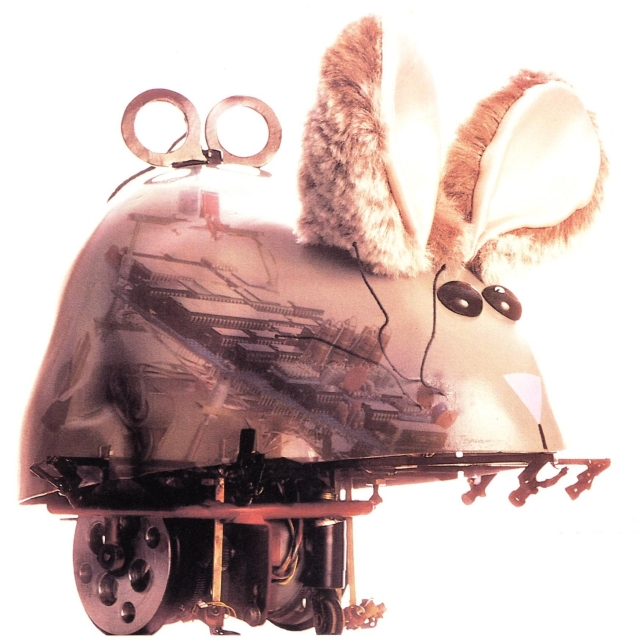
\includegraphics[width=0.6\textwidth]
	{Figures/MoonlightSpecial.jpg}
	\label{fig:MoonlightSpecial}
	\source{\citeonline{Moonlight2010}}
\end{figure}

\hspace{0.5cm} Sua ideia surge em 1977, quando a \textit{IEEE Spectrum Magazine} trouxe pela primeira vez o conceito de robôs autônomos para resolução de labirintos. Pouco tempo depois, sua primeira competição foi realizada, em junho de 1979, na primeira \textit{IEEE Amazing Micromouse Maze Contest} organizada na cidade de Nova York. Rapidamente, o conceito da competição se espalhou e, já no começo da década de 90, vários clubes voltados para Micromouse surgiam em escolas e universidades do mundo todo \cite{Tondr2004}.

\hspace{0.5cm} Atualmente, a \textit{IEEE Micromouse Competition} adota uma configuração que consiste em um labirinto de 16 x 16 blocos. Cada bloco possui 18 x 18 cm. As paredes, que possuem 5 cm de altura, são pintadas de branco de modo a ser reflexiva à luz infravermelha. O chão, por outro lado, é pintado de preto, para que não seja reflexivo. Além disso, os competidores sabem previamente que o \textit{micromouse} tem seu ponto de partida localizado em um dos cantos do labirintos, devendo alcançar o seu centro para terminar o desafio. Com base nisso, os participantes devem usar de algorítimos de busca para explorar o labirinto e encontrar a rota mais otimizada para o ponto de chegada estabelecido pela competição. O robô por sua vez, não pode ter suas dimensões maiores que uma seção de 25 x 25 cm. 
%As regras completas estão dispostas como anexo no final do documento.

%--------- NEW SECTION ----------------------
\section{Robótica e \textit{Frameworks}}
\label{sec:robotic_frameworks}
A palavra robô foi utilizada pela primeira vez em 1921 em uma peça teatral pelo dramaturgo checoslovaco Karel Capek. A origem vem da palavra checa robota que significa “trabalho forçado” e tornou-se popular através de filmes como Metrópolis (1926). O dia em que a terra parou (1951) e Planeta proibido (1956). Apesar da inserção do termo robô ser datada de 1921, registros históricos da antiga civilização grega já propunha o desenvolvimento dos primeiros modelos de robôs. Esses tinham aspecto visual semelhante ao de um humano e ou animal, e utilizavam sistemas de pesos e bombas pneumáticas, porém não tinham nenhuma funcionalidade prática, social, e como a época ainda não existia sistemas de produção complexos, esse robôs também não tinham função voltada à produtividade. Era um mecanismo de simples movimentação e sem nenhuma finalidade real. Algum tempo depois, cientistas árabes se dedicaram em fomentar a idéia e pesquisar sobre atribuir possíveis funções a esses robôs, com objetivo de facilitar as necessidades humanas. Esse pensamento revolucionário foi um grande marco na história da robótica. Segundo (PAPERT, 2008) citado por \citeonline {Mahmud2017}, documentos históricos datados de 1495 revelam que Leonardo Da Vinci ao desenvolver uma grande investigação sobre a anatomia humana, permitiu o desenvolvimento de exemplares de bonecos que obtinham articulações mecânicas, sendo capazes de mover as mãos, cabeça, olhos e pernas, conseguiam até realizar algumas ações mais simples, tal como, escrever ou tocar alguns instrumentos. 

O desenvolvimento produtivo em larga escala dos robôs aconteceu no início do século XVIII com a ascensão da revolução industrial. Segundo (SANTOS; MENEZES, 2005) citado por \citeonline{Mahmud2017}, a indústria têxtil utilizava teares mecânicos e com o contínuo avanço da revolução industrial, as fábricas começaram a substituir algumas tarefas mecanizadas por máquinas capazes de reproduzir automaticamente estas ações.Os anos 30 foram marcados no campo da robótica pela produção de um robô humanoide, denominado de Elektro, produzido pela empresa Westinghouse Electric Corporation. Elektro foi apresentado em 1939 e 1940 na World’s Fair,  uma feira de exposição internacional de produtos manufaturados. Segundo (SILVA, 2009) citado por \citeonline{Mahmud2017}, o termo “robótica” foi enunciado pela primeira vez em 1942 pelo cientista Isaac Asimov, em uma pequena história chamada “Runaround”. Asimov também publicou uma compilação de histórias em 1950 chamada “I Robot”, na qual ele propunha a existência de 3 leis fundamentais aplicadas à robótica, e, posteriormente ele adicionou mais uma, a lei zero. Essas leis são:

\begin{enumerate}
	\item Um robô não pode ferir um ser humano ou, por omissão, permitir que um ser humano sofra algum mal;
	\item Um robô deve obedecer as ordem que lhe sejam dadas por seres humanos, exceto nos casos em que tais ordens contrariem a primeira lei;
	\item Um robô deve proteger sua própria existência desde que tal proteção não entre em conflito com a primeira e segunda lei.
\end{enumerate}

zero.     Um robô não pode fazer mal à humanidade e nem por inação, permitir que ela sofra algum mal.

Porém, atualmente estas leis são interpretadas de uma perspectiva puramente ficcional, afinal, no tempo em que foram formuladas, não se tinha dimensão do desenvolvimento vertiginoso que iria ocorrer na área da robótica.

Apesar de que robôs industriais não se assemelham ao físico humano, ainda assim eles os substituem ao desempenhar tarefas nocivas para as pessoas. O conceito de robô industrial foi patenteado por George Devol, em 1954. O avanço tecnológico permitiu que os robôs passassem a desempenhar funções muito mais complexas e em várias esferas profissionais, por exemplo, indústria automotiva, nuclear, aplicação espacial, aplicação na medicina, em  ambientes adversos, onde a presença humana se torna difícil e até mesmo impossível.

Se tratando de avanço tecnológico, o campo de engenharia de software está ligado diretamente com o desenvolvimento dos robôs atualmente e umas das principais ferramentas de auxílio na programação dos mais diversos tipos de robôs, é o \textit{framework}. Um \textit{framework} pode ser conceituado de algumas formas.	 

Segundo Fayad et al. (1999) e Johnson \& Foote (1988), citado por \citeonline{Junior2006}, “um \textit{framework }é um conjunto de classes que constitui um projeto abstrato para a solução de uma família de problemas.”

Para Mattsson (1992, 2000), citado por \citeonline{Junior2006} “um \textit{framework} é uma arquitetura desenvolvida como objetivo de atingir máxima reutilização, representada como um conjunto de classes abstratas e concretas, com grande potencial de especialização.”
Já para Buschmann et al. (1996), Pree (1995) e Pinto (2000), citado por \citeonline{Junior2006} “um \textit{framework }é definido como um software parcialmente completo projetado para ser instanciado.”

Apesar de diferentes as definições encontradas nas literaturas elas não são contraditórias. A ideia de reutilização de softwares é fundamental para a definição de \textit{framework}, afinal uma ferramenta propõe a execução de uma tarefa de maneira mais prática e rápida. Uma comparação deixando claro as diferenças entre um \textit{framework }e uma biblioteca de classe, pode permitir um melhor entendimento sobre o tema. Numa biblioteca de classes, cada classe é única e independente das outras. Já em um \textit{framework}, as dependências/colaborações estão embutidas, conforme ilustrado na Figura \ref{fig:biblioteca_vs_framework}.

\begin{figure}[H]
	\centering
	\caption{Biblioteca x \textit{Framework}.}
	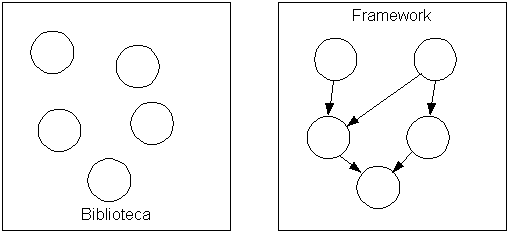
\includegraphics[width=0.7\textwidth]
	{Figures/biblioteca_vs_framework}
	\label{fig:biblioteca_vs_framework}
	\source{\citeonline{Sauve2001}}
\end{figure}

O \gls*{ros} é um exemplo de \textit{framework}. Ele é uma plataforma de software de código aberto, desenvolvido em 2007, projetado para suportar uma nova geração de robôs. A comunidade \gls*{ros} desenvolveu o \textit{framework} para várias plataformas, disponibilizando-os assim para diferentes \gls*{so}, como Windows, Linux e Mac OS. O \gls*{ros} é um conjunto de ferramentas que gerencia de forma eficiente  a mediação entre o SO e demais aplicações, possui uma estrutura flexível permitindo a criação de software de robôs. Detém uma coleção de bibliotecas e convenções com objetivo de simplificar tarefas complexas e criar estruturas mais robustas em uma ampla gama de plataformas robóticas. Pode-se afirmar que o \gls*{ros} representa uma coleção muito útil de softwares voltados exatamente para ajudar na percepção, controle e modelagem dos dispositivos de hardware que serão lidos, fornecendo serviços que são esperados de um SO, incluindo a abstração de hardware em baixo nível, o que permite a leitura e o controle do mesmo, passagem de mensagens entre processos e gerenciamento de pacotes (Quigley et al. 2009, apud \citeonline{Tavares2013}). O \gls*{ros} também disponibiliza ferramentas de aplicação de robótica nas áreas de navegação, simulação, visão, percepção e controle, sendo exemplo as bibliotecas de processamento de imagem (opencv, pcl) e simuladores (stage, gazebo).

Por ser uma plataforma com código aberto, o \gls*{ros} possui uma ampla documentação, bem detalhada, em sua maioria na língua inglesa. Na página da comunidade \gls*{ros}, existe um extenso material de apoio, oferecendo suporte a compartilhamento de códigos fonte e experiências realizadas com o \textit{framework}. A comunidade do \gls*{ros} permite que o usuário faça parte dela, mediante a um cadastro pessoal no site. Dessa forma, o usuário pode deixar eventuais perguntas e/ou dúvidas que poderão ajudá-lo a solucionar algum problema.

O framework \gls*{ros} foi projetado para atender a um conjunto específico de desafios encontrados durante o desenvolvimento de robôs. O \gls*{ros} é muito mais do que apenas um serviço oferecido a robôs móveis e de manipulação (Alexander et al. 2012, apud \citeonline{Tavares2013}).

O \gls*{ros} possui uma estrutura distribuída de processos, a qual apoia a reutilização de código em robótica. Suas bibliotecas possuem funcionalidade para diversas linguagens de programação, foi projetado com um idioma neutro, suportando C, C++, Python, LISP e Octave, apesar de que C++ e Python são as duas linguagens principais e com maior número de pacotes disponíveis. Além disso, O \gls*{ros} organiza seu conjunto de software em \textit{packages} ou pacotes em tradução livre. De acordo com o guia de utilização do \gls*{ros},

\begin{quoting}[rightmargin=0cm,leftmargin=4cm]
	\begin{singlespace}
		{\footnotesize
			[...]um pacote pode conter nós \gls*{ros}, uma biblioteca independente de \gls*{ros}, um conjunto de dados, arquivos de configuração, um software de terceiros ou qualquer outra coisa que constitua logicamente um módulo útil. O objetivo desses pacotes é fornecer essa funcionalidade útil de maneira fácil de consumir, para que o software possa ser facilmente reutilizado. Em geral, os pacotes \gls*{ros} seguem o princípio "Goldilocks": funcionalidade suficiente para ser útil, mas não muito que o pacote seja pesado e difícil de usar em outro software. \cite[tradução nossa]{rospackages}
		}
	\end{singlespace}
\end{quoting}


A comunicação do \gls*{ros} é baseada em eventos, utiliza processos para publicar/subscrever nós a tópicos. Conceitualiza-se que os nós publicam e subscrevem os tópicos, permitindo assim uma comunicação entre nós, onde recebem mensagens, apenas os que estiverem subscritos ao tópico.

A Figura \ref{fig:estrutura_comunicacao_ros} demonstra uma simples publicação e subscrição de dois nós a um tópico. Desta forma sempre que o nó publicar novas mensagens os nós que estejam subscritos ao tópico irão receber a informação.

\begin{figure}[H]
	\centering
	\caption{Estrutura de comunicação.}
	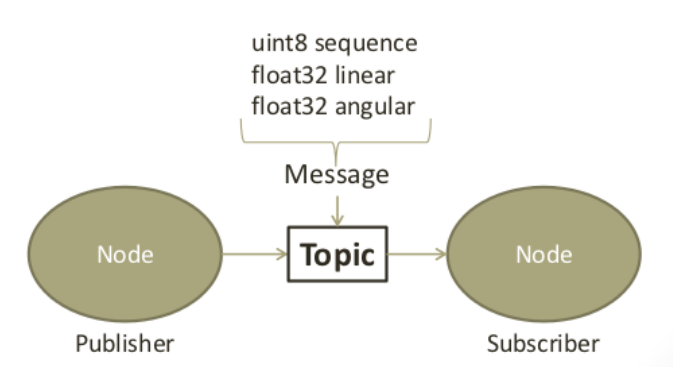
\includegraphics[width=0.7\textwidth]
	{Figures/estrutura_comunicacao_ros}
	\label{fig:estrutura_comunicacao_ros}
	\source{\citeonline{Santos2013}}
\end{figure}

Os nós correspondem à execução de um programa e são criados no sistema, geralmente, via console e sempre com o servidor mestre \gls*{ros} (roscore) iniciado. O servidor roscore é responsável por inicializar várias dependências, bibliotecas do \gls*{ros} e o sistema de comunicação entre nós. Devida as vantagens descritas neste tópico, será utilizado o \textit{framework} ROS para o desenvolvimento do Doogie Mouse.
%--------- NEW SECTION ----------------------
\section{Estudo do Estado da Arte}
\label{sec:sota}
Nessa seção, será realizado um estudo comparativo de alguns modelos de \textit{micromouse}, buscando avaliá-los sobre diferentes critérios a partir de uma matriz de comparação. O estudo auxiliou na realização do design da paltaforma proposta por esse trabalho uma vez que, através dele, verifica-se quais recursos são mais importantes para o comprimento dos requisitos do projeto, além de permitir um entendimento generalizado de como são feitos os robôs \textit{micromouse}. 

\subsection{GreenGiant}
A Green Giant é uma desenvolvedora de múltiplas plataformas de robótica, especializada em eletrônica embarcada, tendo como seu carro-chefe o \textit{micromouse}. Seu modelo mais recente, 2016 - 2017, é voltado para alto desempenho em competições, alcançando a posição de quarto lugar durante a \gls*{apec} de 2016.

\begin{figure}[H]
	\centering
	\caption{Robô Green Giant.}
	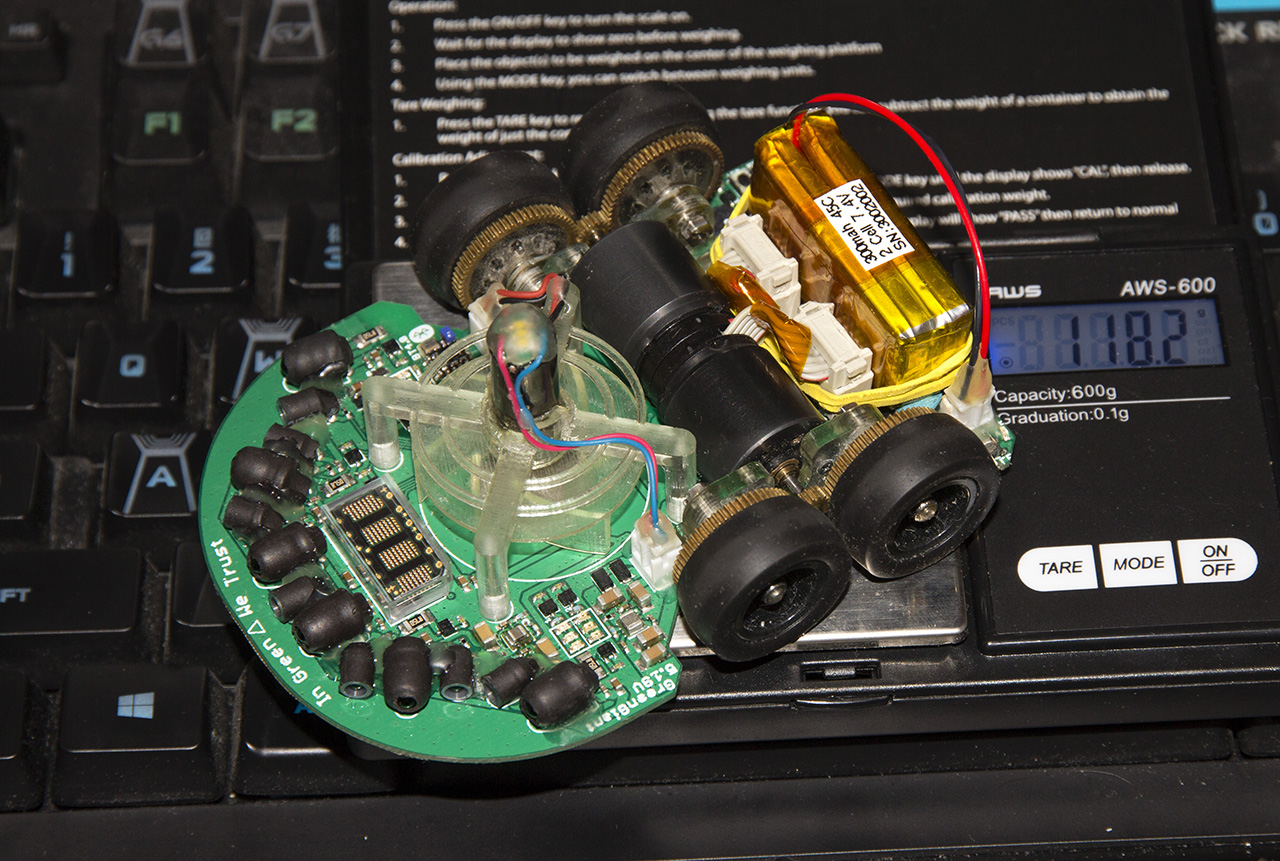
\includegraphics[width=0.7\textwidth]
	{Figures/GreenGiant_model.jpg}
	\label{fig:Green_Giant_model}
	\source{\citeonline{GreenGiant2016}}
	\end{figure}

Sua interface de usuário possui \textit{Dot Matrix Display}, sinalizadores LED, botões, buzzer, além de possuir um sistema de comunicação Bluetooth 4.0. Ademais, o modelo usa um sistema de ventoinhas de sucção para aumentar o nível de aderência das rodas, permitindo alcançar maiores velocidades sem derrapar.


\begin{table}[H]
	\centering
	\caption{Atributos do robô Green Giant}
	\label{tab:Green_Giant}
	\begin{tabular}{|l|l|}
		\hline
		\multicolumn{2}{|l|}{\textbf{Green Giant 5.19V}} \\ \hline
		Fabricante & Green Ye \\ \hline
		Ano & 2017 \\ \hline
		Linguagem de Programação & C/C++ \\ \hline
		Sensores & IR, MPU, IE \\ \hline
		Controlador & STM32 \\ \hline
		Simulador & - \\ \hline
		Bateria & LiPo 300mAh (7,4V) \\ \hline
		Rodas & 3D printed mount\&wheel + mini-z tyres \\ \hline
		Motor & DC-Motor 6.540RPM 0,21N.m (6V) \\ \hline
		User Interface & DMD 5x7, LEDs, Botão, Bluetooth \\ \hline
		Outros & sistema de ventoinhas de sucção \\ \hline
	\end{tabular}
	\source{Adaptado de \citeonline{GreenGiant2016}}
\end{table}


\textbf{Pontos Positivos:}
\begin{itemize}
	\item Produto de alto desempenho em competições;
	\item Sistema de ventoinhas de sucção.
\end{itemize}


\textbf{Pontos Negativos:}
\begin{itemize}
	\item Não possui suporte à simulação;
	\item Projeto pouco documentado;
	\item Não possui guia do usuário;
	\item Não possui suporte nativo para ambiente \gls*{ros}.
\end{itemize}


\subsection{WPISmartMouse}
A organização estudantil, WPI CollabLab, compartilham um espaço de laboratório entre seus membros para projetos com viez colaborativo a sociedade. Nesse espaço desenvolveu-se o Smartmouse, projeto \textit{micromouse} voltado para a competição Micromouse \textit{Brown IEEE Robotic  Olympiad}. O projeto também se extendeu para o desenvolvimento de um ambiente de simulação apartir dos projetos Gazebo e Ignition, não possuindo entretanto suporte para \gls*{ros}.

\begin{figure}[H]
	\centering
	\caption{Robô WPISmartMouse}
	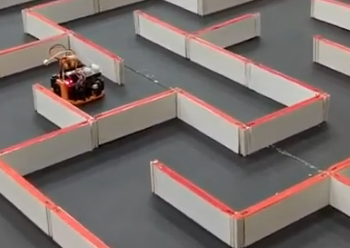
\includegraphics[width=0.5\textwidth]
	{Figures/WPISmartMouse_model.png}
	\label{fig:WPISmartMouse_model}
	\source{\citeonline{WpiSmartMouse2017}}
\end{figure}

\begin{table}[H]
	\centering
	\caption{Atributos do robô WPISmartmouse}
	\begin{tabular}{|l|l|}
		\hline
		\multicolumn{2}{|l|}{\textbf{Smartmouse}} \\ \hline
		Fabricante & WPI CollabLab \\ \hline
		Ano & 2018 \\ \hline
		Linguagem de Programação & Arduino/C, Python, BASCOM \\ \hline
		Sensores & IR, Magnetic Encoder \\ \hline
		Controlador & Teensy 3.6 \\ \hline
		Simulador & Gazebo \\ \hline
		Bateria & LiPo 1500mAh (7,4V) \\ \hline
		Rodas & Solarbotics RW2i Wheel \\ \hline
		Motor & DC-Motor 650RPM 2,35Nm(6V) \\ \hline
		User Interface & LEDs \\ \hline
		Outros & documentação no git \\ \hline
	\end{tabular}
	\label{tab:Smartmouse}
	\source{Adaptado de \citeonline{WpiSmartMouse2017}}
\end{table}

\textbf{Pontos Positivos:}
\begin{itemize}
	\item Provê ambiente de simulação;
	\item Documentação disponível no GitHub;
	\item Possui portabilidade para mais de uma linguagem de programação.
\end{itemize}

\textbf{Pontos Negativos:}
\begin{itemize}
	\item Não possui suporte nativo para ambiente \gls*{ros};
	\item Pouca variedade de sensores;
	\item Não possui guia do usuário;
	\item Poucos recursos na interface com o usuário.
\end{itemize}


\subsection{Kumamoto National College}
O Instituto Nacional de Tecnologia de Kumamoto, \textit{Kumamoto National College}, apresentou no ano de 2008 um projeto de desenvolvimento de ferramentas educacionais voltada para integração de sistemas e suas implementações. O projeto é direcionado aos seus estudantes do 5º ano de engenharia, através da produção de um \textit{micromouse} para a competição do ramo de \textit{Kyushu}.

\begin{figure}[H]
	\centering
	\caption{Robô Kumamoto.}
	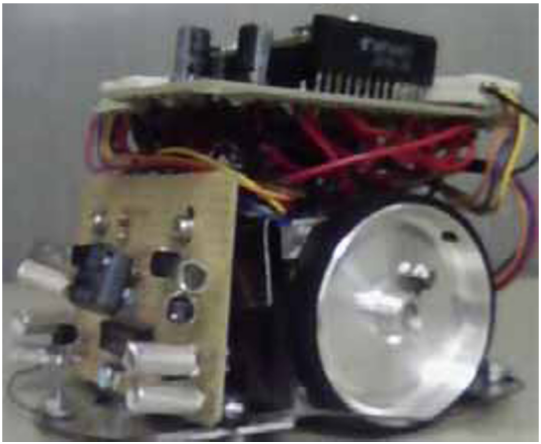
\includegraphics[width=0.5\textwidth]
	{Figures/Kumamoto_model.png}
	\label{fig:Kumamoto_model}
	\source{\citeonline{Kumamoto2010}}
\end{figure}

O hardware do robô foi bastante simplificado, visando facilitar o desenvolvimento pelos estudantes ainda não familiarizados com a robótica e eletrônica, além de buscar reduzir os custos de produção do robô. Como ferramenta educativa, o projeto conseguiu que seus estudantes produzissem o \textit{micromouse} em um semestre de atividades. Contudo, conceitos da robótica (ex: robótica móvel, fusão de sensores, visão, navegação) não foram trabalhados ou não foram citados no artigo gerado a partir do projeto.


\begin{table}[H]
	\centering
	\caption{Atributos do robô Kumamoto}
	\begin{tabular}{|l|l|}
		\hline
		\multicolumn{2}{|l|}{\textbf{Kumamoto National College}} \\ \hline
		Fabricante & Kiyoteru Hayama and Tsutomu Matsumoto \\ \hline
		Ano & 2008 \\ \hline
		Linguagem & C \\ \hline
		Sensores & IR \\ \hline
		Controlador & H8Tiny-3664 \\ \hline
		Simulador & - \\ \hline
		Bateria & LiPo 900mAh (7,4V) \\ \hline
		Rodas & wheels, tires \\ \hline
		Motor & Step Motor 0,78Nm (5,6V) \\ \hline
		User Interface & LEDs \\ \hline
		Outros & Documentação em artigo \\ \hline
	\end{tabular}
	\label{tab:Kumamoto}
	\source{Adaptado de \citeonline{Kumamoto2010}}
\end{table}



\textbf{Pontos Positivos:}
\begin{itemize}
	\item Projeto com fins educacionais;
	\item Fácil desenvolvimento.
\end{itemize}

\textbf{Pontos Negativos:}
\begin{itemize}
	\item Não possui suporte nativo para ambiente \gls*{ros};
	\item Pouca variedade de sensores;
	\item Não possui guia para usuário;
	\item Poucos recursos na interface com o usuário;
	\item Não possui nenhum ambiente de simulação.
\end{itemize}


\subsection{WolfieMouse}
\hspace{0.5cm} O WolfieMouse é um projeto de robótica que desenvolveu um \textit{micromouse} para competir na \textit{2018 Region 1 Robotics Competition}.

\begin{figure}[H]
	\centering
	\caption{Robô WolfieMouse.}
	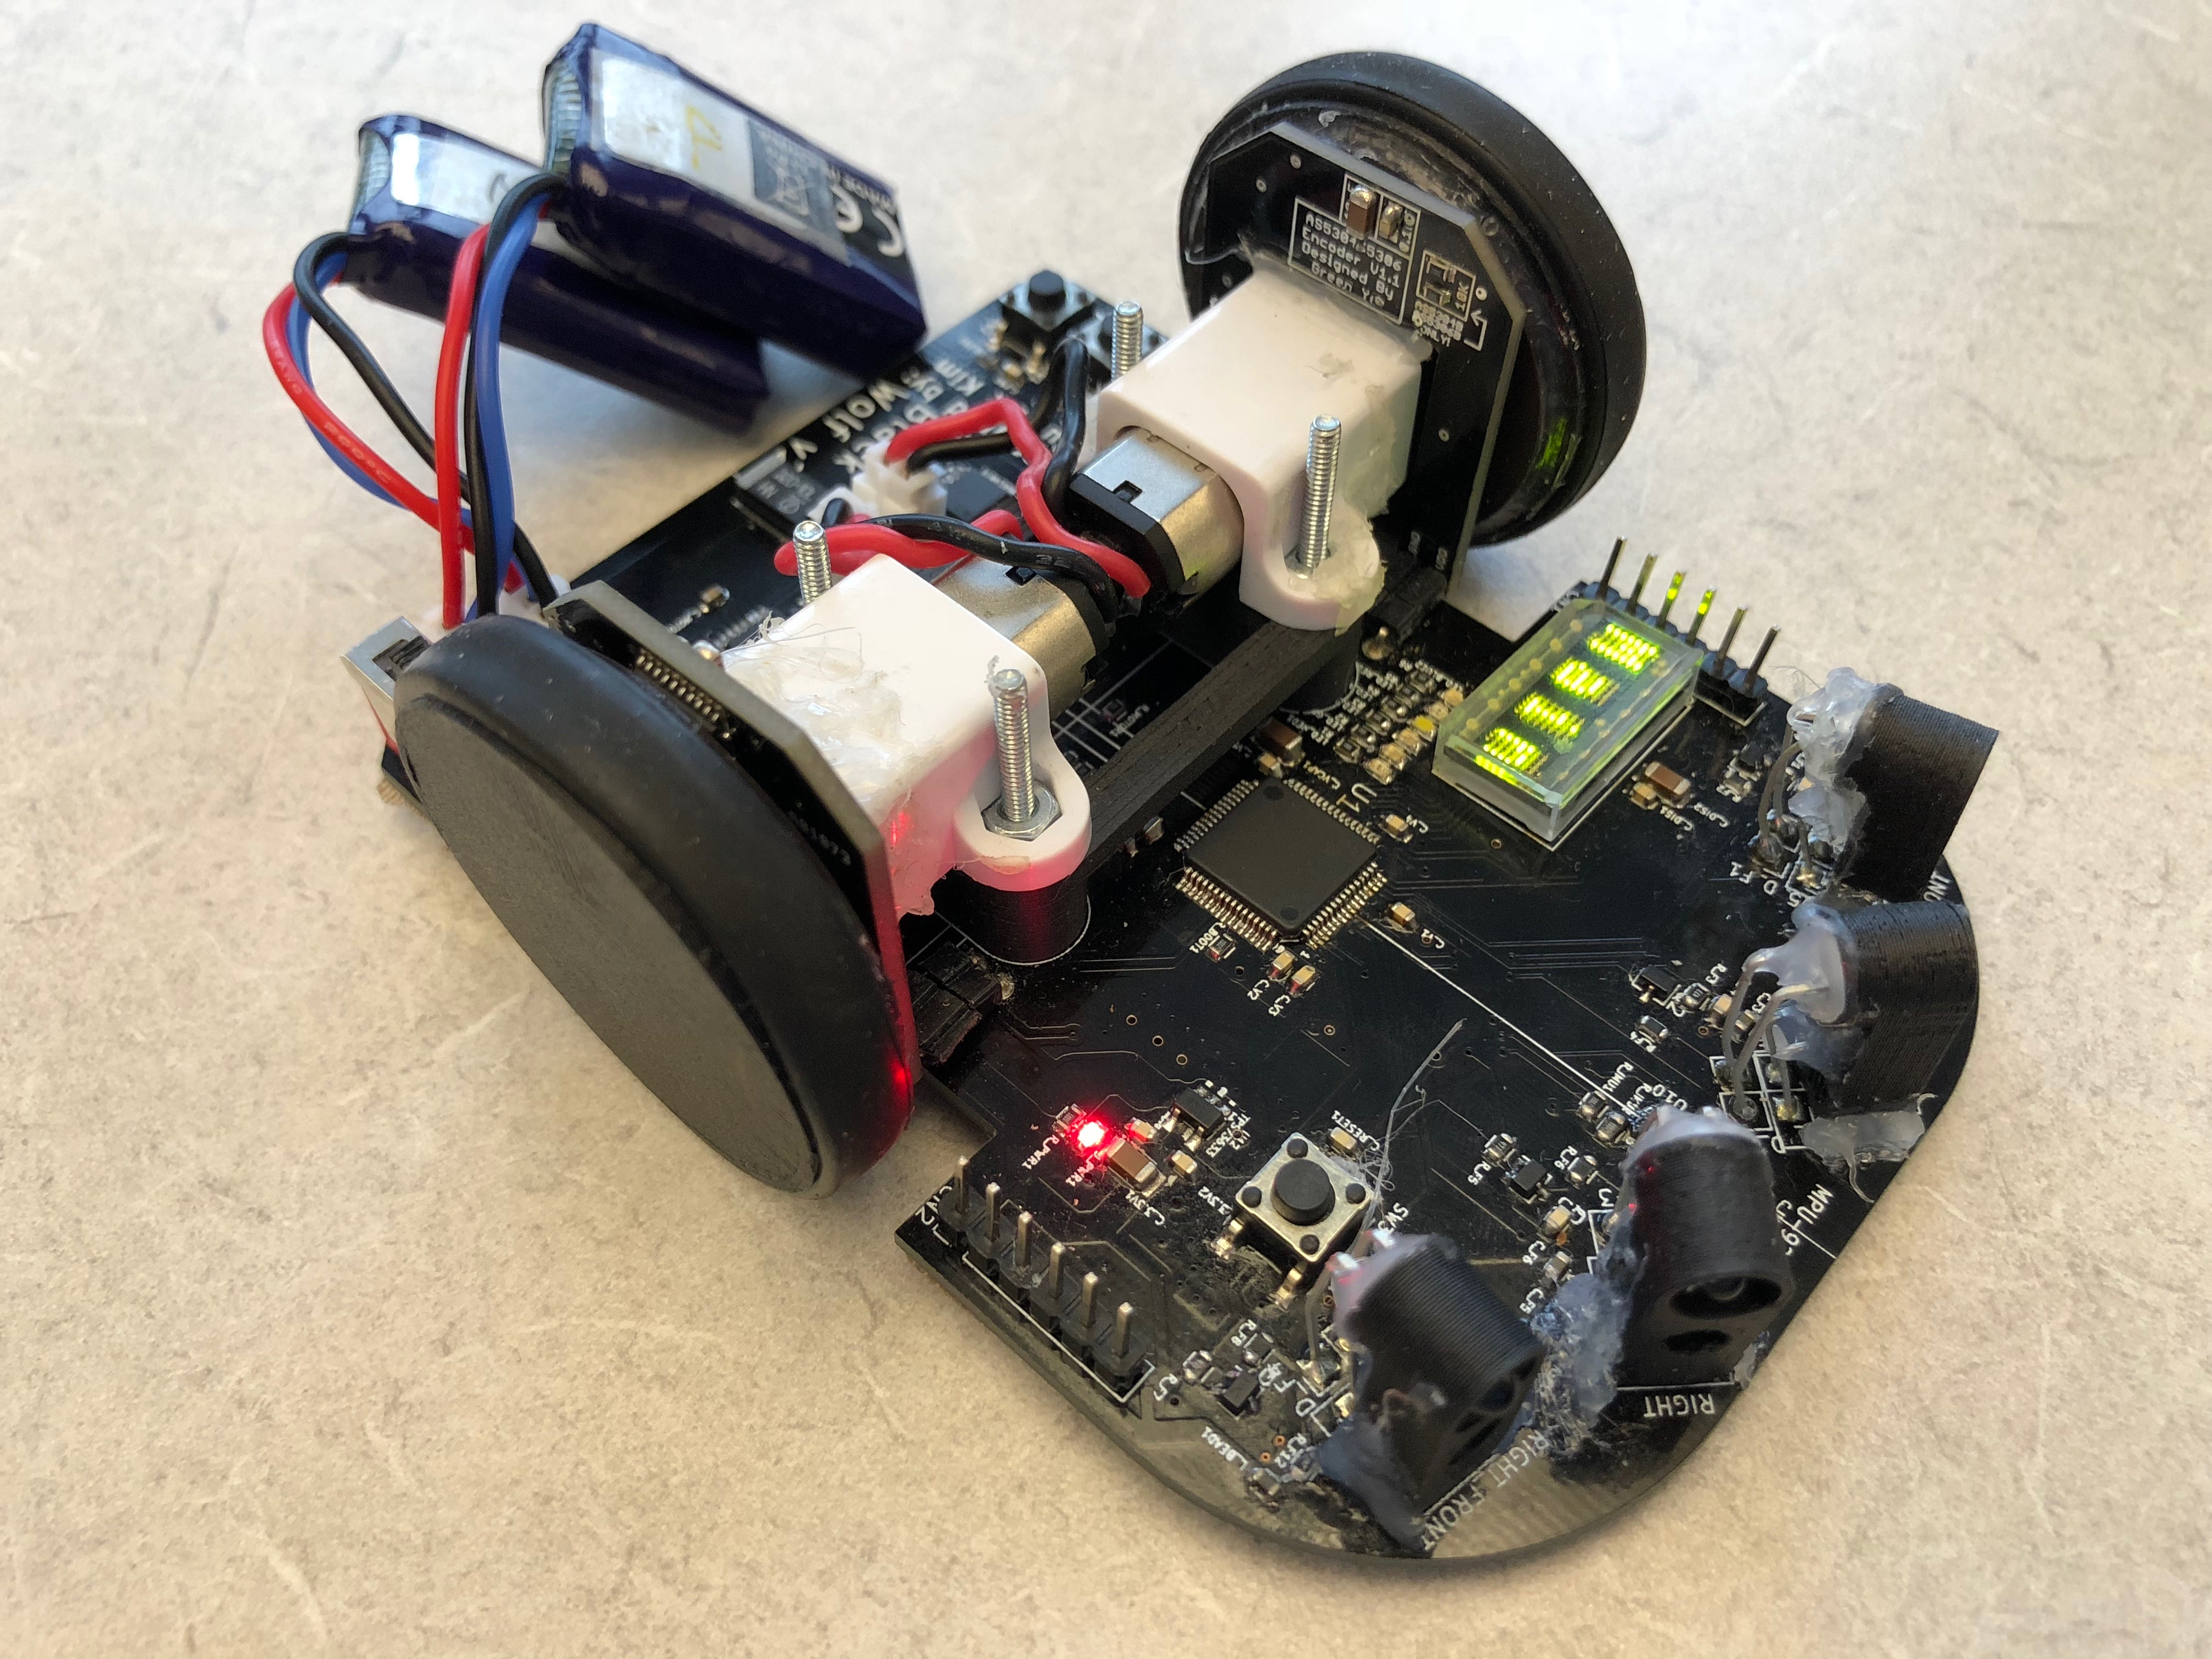
\includegraphics[width=0.7\textwidth]
	{Figures/WolfieMouse_model.jpg}
	\label{fig:WolfieMouse_model}
	\source{\citeonline{WolfieMouse2018}}
\end{figure}

Além da plataforma robótica, que conta com hardwares programados em baixo nível, para melhor otimização de seus controles, a equipe também realizou um ambiente de simulação baseado em C++ emulado no terminal do computador. Toda documentação foi disponibilizada em um repositório git, que também possui tutoriais para o desenvolvimento do robô.

\begin{table}[H]
	\centering
	\caption{Atributos do robô WolfieMouse}
	\begin{tabular}{|l|l|}
		\hline
		\multicolumn{2}{|l|}{\textbf{WolfieMouse}} \\ \hline
		Fabricante & Bryant Gonzaga, Bum Kim, Hyun Choi \\ \hline
		Ano & 2018 \\ \hline
		Linguagem & C++, C, ARM Assembly, Python \\ \hline
		Sensores & MPU, ToF, Magnetic Encoder \\ \hline
		Controlador & STM32 \\ \hline
		Simulador & Terminal-based \\ \hline
		Bateria & * \\ \hline
		Rodas & * \\ \hline
		Motor & DC-Motor \\ \hline
		User Interface & DMD 5x7, botões \\ \hline
		Outros & documentação e tutoriais no git \\ \hline
	\end{tabular}
	\label{tab:WolfieMouse}
	\source{Adaptado de \citeonline{WolfieMouse2018}}
\end{table}

\textbf{Pontos Positivos:}
\begin{itemize}
	\item Projeto bem documentado;
	\item Possui tutoriais;
	\item Possui ambiente de simulação.
\end{itemize}

\textbf{Pontos Negativos:}
\begin{itemize}
	\item Não possui suporte nativo para ambiente \gls*{ros};
	\item Pouco foco em finalidades educativas com o produto;
	\item Não possui guia para usuário;
	\item Poucos recursos na interface com o usuário.
\end{itemize}

\subsection{Raspberry Pi Mouse V2}
A RT Corporation Micromouse é uma desenvolvedora japonesa de plataformas robóticas voltada para aplicações  voltadas de pesquisas à hobistas. Um de seus segmentos é voltado para \textit{micromouse}, fortemente representado pelo seu produto Raspberry Pi Mouse V2, citado em "Learning ROS robot programming with Raspberry Pi" (Nikkei BP, June 2018).

\begin{figure}[H]
	\centering
	\caption{Robô RaspiMouse.}
	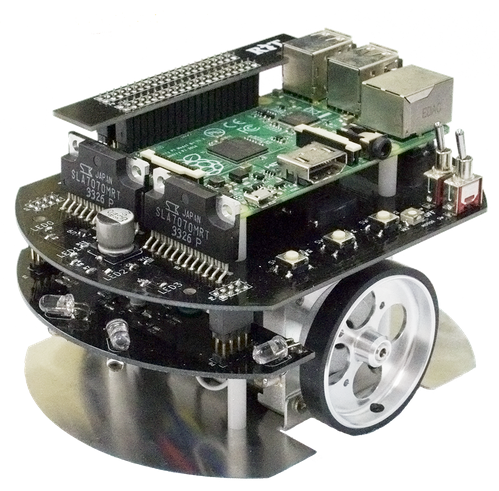
\includegraphics[width=0.5\textwidth]
	{Figures/RaspiMouse_model.png}
	\label{fig:RaspiMouse_model}
	\source{\citeonline{RaspiMouse2016}}
\end{figure}

O modelo citado, é um robô de plataforma baseado em \textit{micromouse} que utiliza uma Raspberry Pi como sua placa principal. Dessa forma o robô pode ser controlado pelos principais \textit{middleware} de robótica (ROS/RTM), possuindo inclusive pacotes publicados na wiki do \gls*{ros} voltados para navegação e simulação do \textit{micromouse};

\begin{table}[]
	\centering
	\caption{Atributos do robô RaspiMouse}
	\begin{tabular}{|l|l|}
		\hline
		\multicolumn{2}{|l|}{\textbf{Raspberry Pi Mouse V2}} \\ \hline
		Fabricante & RT Corporation \\ \hline
		Ano & 2016 \\ \hline
		Linguagem & Python, Shell \\ \hline
		Sensores & IR \\ \hline
		Controlador & RaspberryPi3 \\ \hline
		Simulador & Gazebo \\ \hline
		Bateria & LiPo 1000mAh (7,4V) \\ \hline
		Rodas & wheels, tires \\ \hline
		Motor & Step-Motor 400step/rev (4 fases) \\ \hline
		User Interface & Terminal, LEDs, Botão, Buzzer \\ \hline
		Outros & documentação no Git, mas em japonês \\ \hline
	\end{tabular}
	\label{tab:RaspiMouse}
	\source{Adaptado de \citeonline{RaspiMouse2016}}
\end{table}

\textbf{Pontos Positivos:}
\begin{itemize}
	\item Projeto bem documentado;
	\item Disponível no GitHub;
	\item Possui tutoriais;
	\item Possui ambiente de simulação;
	\item Suporte aos principais middleware de robótica (ROS/RTM);
	\item Possui pacotes do \gls*{ros} para seu controle;
	\item Plataforma é expansível.
\end{itemize}

\textbf{Pontos Negativos:}
\begin{itemize}
	\item Toda documentação do produto está em japonês;
	\item O robô é pouco compacto.
\end{itemize}

\subsection{Matriz de Comparação}

Através do estudo conforme tópico anteriores, montou-se uma matriz de comparação de forma a
quantificar atributos considerados mais significativos para o robô. Levou- se em conta, portanto, a existência da documentação disponível e seu nível de clareza; o uso de algum \textit{framework} de robótica; se faz uso ou suporta algum ambiente de simulação; diversidade de linguagens que a
plataforma pode ser programada; como é realizada a interface do usuário; quantidade de diferentes sensores e se a plataforma é expansível, podendo acrescentar a ela outros recursos (seja em hardware ou em software). Essa matriz pode ser visualizada no Apêndice \ref{apend:matriz_de_comparacao} deste documento.